% =====================================================================
% Paper 19 - The Two-Sided Cost of CMDB Error: Ghost Assets, Phantom
% Assets, and the Matching-Precision Ceiling of Self-Healing
% Reconciliation. IEEE TNSM submission. Build with tectonic.
% Reproducibility: results/primary_v1/ (frozen on seeds 1300-1324).
% Run src/run_evaluation.py.
% =====================================================================
\documentclass[journal]{IEEEtran}

\usepackage{graphicx}
\usepackage{booktabs}
\usepackage{amsmath}
\usepackage{amssymb}
\usepackage{newtxtext,newtxmath}
\usepackage{hyperref}
\usepackage{xurl}
\usepackage{url}
\usepackage{array}

\graphicspath{{figures/}}

\title{The Two-Sided Cost of CMDB Error: Ghost Assets, Phantom Assets, and the\\
Matching-Precision Ceiling of Self-Healing Reconciliation}

\author{%
  \IEEEauthorblockN{Harshavardhan Malla}
  \IEEEauthorblockA{Independent Researcher\\ Email: harshavardhanmalla75@gmail.com}%
}

\renewcommand{\textendash}{-}
\renewcommand{\textemdash}{-}
\usepackage{etoolbox}
\makeatletter
\patchcmd{\abstract}{---}{:\space}{}{}
\patchcmd{\IEEEkeywords}{---}{:\space}{}{}
\makeatother
\begin{document}
\maketitle

\begin{abstract}
A configuration management database is the asset inventory on which security and cost management
both depend, and it is never accurate because the fleet churns faster than it is reconciled. Its
errors are two-sided: a ghost asset, meaning a real asset missing from the inventory, is a security
cost, and a phantom asset, meaning a record with no real asset behind it, is a financial and noise
cost. The two errors have opposite remedies, so reducing one tends to raise the other, and the
operating point that minimizes their sum is not at either extreme. We quantify both errors with a
pre-registered simulation of a churning fleet, with hypotheses, thresholds, and evaluation seeds
locked before any result was inspected. Continuous self-healing reconciliation reduces total
inventory error from 0.6047 under quarterly reconciliation to 0.1342, a reduction of 0.778 (95\%
bias-corrected and accelerated bootstrap interval $[0.7765, 0.7795]$), almost all of it by closing
the discovery lag that leaves new assets as ghosts. The two errors trade off against retirement
aggressiveness: lengthening the retirement threshold from 7 to 120 days drops the ghost rate from
0.1025 to 0.0075 but raises the phantom rate from 0.0598 to 0.3696, so total error has an interior
minimum at a threshold of 14 days. The accuracy floor is set by record-matching precision:
duplicate records from failed matches persist regardless of cadence, and total error falls from
0.2831 to 0.0954 as precision rises from 0.80 to 0.99, against a duplicate-driven floor proxy of
0.1877. The cost-minimizing threshold is 30 days when ghosts are weighted five to one over phantoms,
14 days when the two are balanced, and 7 days when phantoms are weighted five to one. Reconcile
continuously, tune the retirement threshold to the interior optimum set by the security-to-cost
balance, and invest in the matcher, because matching precision sets a floor that no cadence can beat.
A closed-form analysis derives each of these shapes from the reconciliation accounting: the ghost rate
decays onto a discovery-lag floor, the phantom rate rises linearly above an irreducible duplicate floor
of one minus the matching precision, their sum is U-shaped with an interior minimum, and the
cost-weighted optimum shifts monotonically with the ghost-to-phantom cost ratio. An adversarial reading
follows, since an attacker who keeps an asset quiet manufactures a ghost on purpose, so a
security-weighted program must run a lenient retirement threshold to keep quiet assets in the inventory.
\end{abstract}

\begin{IEEEkeywords}
CMDB, asset inventory, configuration management, record linkage, entity resolution, ghost assets,
phantom assets, self-healing reconciliation, pre-registration, reproducibility
\end{IEEEkeywords}

\section{Introduction}
\IEEEPARstart{A}{configuration} management database (CMDB) is the authoritative record of what an
organization owns and operates, and an accurate asset inventory is a security control in its own
right~\cite{nist80053,cisabod2301}. Almost every other control depends on it. An asset the inventory
does not know about is not patched, not monitored, not scanned, and not protected; an asset the
inventory records but that no longer exists drives spending on licenses and agents that touch
nothing and generates alerts that mean nothing. Continuous monitoring guidance makes the inventory a
living object rather than an annual snapshot~\cite{nist80137,nist80137a}, and a federal directive now
binds agencies to maintain visibility of the assets on their networks~\cite{cisabod2301}. Yet the
inventory is never perfectly accurate, for a structural reason: the real fleet churns. Assets are
provisioned and decommissioned continuously, and the inventory is reconciled against reality only as
often as a discovery scan runs and a record is updated. Between scans, reality moves on and the
record falls behind.

The errors that result are two-sided, and the two sides have opposite remedies. We use two terms
throughout. A \emph{ghost} is a live asset that has no active record, so the inventory is blind to
it; a ghost is a security cost,
because a missing asset escapes every control keyed to the inventory. A \emph{phantom} is a record
with no real asset behind it, including a
record left over after an asset is gone and a duplicate created by a failed match; a phantom is a
financial and noise cost. The total error of an inventory is the ghost rate plus the phantom rate.
The crucial property is that the two errors pull against each other. Aggressively retiring records
that have not been observed recently removes phantoms but risks deleting real-but-quiet assets,
turning them into ghosts. Aggressively adding every discovery removes ghosts but, when the matching
that links a fresh observation to its existing record is imperfect, creates duplicate records, which
are phantoms. This is a classical record-linkage problem~\cite{fellegi1969linkage,christen2012matching}
sitting underneath an operational reconciliation loop.

Self-healing reconciliation, meaning continuous discovery paired with confidence-based matching and
automatic correction in the spirit of autonomic computing~\cite{kephart2003vision}, promises to
reduce both errors at once by shrinking the lag that drives them. The promise is real but bounded.
The bound is the precision of the matcher: a fraction of observations will fail to link to the
correct existing record, producing duplicate phantoms that no cadence and no retirement policy can
remove, because they are the result of a matching failure rather than a timing failure. Matching
precision therefore sets a floor on inventory accuracy that operational tuning cannot cross.

This paper quantifies the benefit and its bounds. We do not claim to measure any particular
organization's inventory; we build a transparent model of a churning fleet under reconciliation,
lock a set of hypotheses and thresholds before looking at the evaluation data, and report what the
model says. The contribution is fourfold.

\begin{itemize}
\item We separate the two reconciliation regimes and measure that \emph{continuous} self-healing
reconciliation cuts total inventory error far below \emph{quarterly} periodic reconciliation, almost
entirely by removing the discovery-lag ghosts that dominate the periodic regime.
\item We characterize the \emph{ghost-phantom tradeoff} that the retirement threshold controls and
show that total error has an \emph{interior minimum}: neither the most aggressive nor the most
lenient retirement is best, because the two errors move in opposite directions across the sweep.
\item We establish a \emph{matching-precision floor}: total error falls as the matcher improves, and
the duplicate records from failed matches form a residual that no cadence or threshold can lower, so
the matcher, not the cadence, sets the achievable accuracy.
\item We show the cost-weighted optimum \emph{shifts with the mission}: the cost-minimizing
retirement threshold moves with the ghost-to-phantom cost ratio, so a security-weighted program and
an availability-weighted program should not run the same retirement policy.
\end{itemize}

The methodology is deliberately conservative. Every quantitative claim is a pre-registered
hypothesis evaluated on seeds that were not inspected during model development, and every interval is
a bias-corrected and accelerated (BCa) bootstrap interval~\cite{efron1987bca,efron1994introduction}
rather than a null-hypothesis significance test, following the pre-registration discipline now
standard in empirical software engineering~\cite{wohlin2012experimentation}.

\section{Background and Related Work}

\subsection{Record linkage, entity resolution, and data matching}
Linking observations of the same real-world entity across noisy records is the subject of record
linkage, founded by the probabilistic theory of Fellegi and Sunter~\cite{fellegi1969linkage} and
developed into the modern field of entity resolution and data matching catalogued by
Christen~\cite{christen2012matching}. The central quantity in that literature is matching precision:
the probability that two records judged to be the same entity actually are, with its complement
producing either missed links or false merges. CMDB reconciliation is record linkage applied to a
moving target. A discovery scan emits an observation that must be linked to the correct existing
record; when the link fails, a duplicate record is created, and a duplicate with no distinct real
asset behind it is precisely a phantom. We import the matching-precision parameter from this
literature and trace its effect through to inventory accuracy, treating the reconciliation loop as an
online entity-resolution problem rather than a one-shot deduplication.

\subsection{Autonomic self-healing and continuous correction}
The autonomic-computing vision of self-managing systems~\cite{kephart2003vision} framed the shift
from periodic human intervention to continuous machine self-assessment and self-correction.
Self-healing reconciliation is an instance: the system continuously discovers, matches, and corrects
its own inventory without waiting for a scheduled audit. The author's prior self-healing remediation
framework for endpoint fleets~\cite{paper10autoheal} applies the same loop to cyber-hygiene
correction. Our contribution here is to quantify where the self-healing loop helps and where it
saturates: it removes the timing-driven component of inventory error but cannot cross the floor set
by the matcher, so the autonomic loop and the record-linkage quality are complementary levers, not
substitutes.

\subsection{Federal asset visibility and configuration data quality}
Maintaining an accurate inventory of authorized assets is mandated rather than optional. NIST SP
800-53~\cite{nist80053} carries the system-component-inventory control, FIPS 199~\cite{fips199} sets
the categorization that scopes which assets matter, and continuous monitoring
guidance~\cite{nist80137,nist80137a} reframes inventory accuracy as an ongoing program rather than a
point-in-time check. CISA Binding Operational Directive 23-01~\cite{cisabod2301} binds federal
agencies to discover and maintain visibility of the assets on their networks on a defined cadence,
which is exactly the reconciliation problem we model. The broader question of database and
configuration data quality, including the security consequences of stale or wrong
data~\cite{bertino2005database}, sits underneath: an inventory is a database whose value collapses
when its records diverge from reality. Breach data continues to attribute incidents to unmanaged and
unknown assets~\cite{verizon2026dbir}, the operational manifestation of the ghost error, and the
author's prior work on hygiene-augmented vulnerability
prioritization~\cite{paper4hygieneprio}, together with the author's earlier context-aware
vulnerability-prioritization study for government endpoint fleets, depends on the inventory being
right in the first place, since an asset absent from the inventory is absent from every
prioritization that reads it.

\section{System Model}
We model a single fleet over a long horizon and measure, at steady state, how much inventory error
each reconciliation regime leaves behind. All quantities are synthetic with documented
distributions; no operational, employer, or inventory data is used.

\subsection{Fleet dynamics}
The fleet is a population of assets in steady state. Each asset has an exponential lifetime with mean
$L = 365$ days, and arrivals are timed so that the live population stays in steady state: as assets
are decommissioned, new assets are provisioned to replace them. The churn rate is therefore set by
$L$; a fleet that turns over once a year is the reference. An asset is \emph{live} from its
provisioning to its decommissioning and is \emph{gone} thereafter.

\subsection{Reconciliation and observation}
Reconciliation runs a discovery scan every reconciliation cadence. We evaluate two regimes:
\emph{continuous} self-healing reconciliation scans every $C_{\text{cont}} = 1$ day, and
\emph{periodic} quarterly reconciliation scans every $C_{\text{quart}} = 90$ days. A scan does not
see every live asset. Each scan observes a given live asset with an observability probability that
encodes that some assets are quiet: assets are seen probabilistically, so even a live asset can go
several scans unobserved, and a quiet asset is at risk of being wrongly retired.

A CMDB record is created when an asset is first observed. A record is \emph{retired} when its asset
has not been observed for the retirement threshold $T$ days, marking it as gone. The threshold is the
central control: a short $T$ retires aggressively, a long $T$ retires leniently.

\subsection{Matching}
At each observation, discovery must link the observed asset to its existing record. The link succeeds
with the \emph{matching precision} $p$ (reference $p = 0.95$); with probability $1 - p$ the match
fails and a duplicate record is created. A duplicate has no distinct real asset behind it and is
therefore a phantom; it persists until it is itself retired for non-observation. The matching
precision is the record-linkage quality of the discovery pipeline~\cite{fellegi1969linkage,christen2012matching}
and is the only lever that acts on the duplicate component of the phantom error.

\subsection{Error definitions and objective}
Two errors are measured at steady state. The \emph{ghost rate} $g$ is the fraction of the live fleet
with no active CMDB record, comprising newly provisioned assets not yet discovered and
real-but-quiet assets that were wrongly retired:
\begin{equation}
g \;=\; \frac{\#\{\text{live assets with no active record}\}}{\#\{\text{live assets}\}}.
\label{eq:ghost}
\end{equation}
The \emph{phantom rate} $\phi$ is the number of CMDB records with no corresponding live asset,
counting both records of gone assets not yet retired and duplicate records from failed matches,
expressed as a fraction of the live fleet:
\begin{equation}
\phi \;=\; \frac{\#\{\text{records of gone assets}\} + \#\{\text{duplicate records}\}}{\#\{\text{live assets}\}}.
\label{eq:phantom}
\end{equation}
The \emph{total error} is their sum, $\epsilon = g + \phi$, and is the quantity a regime is judged
by when ghosts and phantoms are treated as equally costly. When they are not, the operating point is
chosen by the \emph{cost-weighted error}
\begin{equation}
\epsilon_w \;=\; w_g \, g \;+\; w_\phi \, \phi,
\label{eq:costweighted}
\end{equation}
where $w_g$ is the cost of a ghost (a security cost) and $w_\phi$ the cost of a phantom (a financial
and noise cost). The balanced case $w_g = w_\phi$ recovers the total error; a security-weighted
program sets $w_g > w_\phi$, and an availability- or cost-weighted program sets $w_g < w_\phi$. The
retirement threshold $T$ that minimizes $\epsilon_w$ is the operating point, and the model's claim is
that it moves with the ratio $w_g / w_\phi$.

\subsection{Sweeps}
The retirement threshold is swept over $T \in \{7, 14, 30, 60, 120\}$ days and the matching precision
over $p \in \{0.80, 0.90, 0.95, 0.99\}$. Errors are estimated by per-asset Monte Carlo over the
fleet at steady state.

\section{Experimental Design}
The study is pre-registered. Hypotheses, thresholds, model constants, and the evaluation seed range
were fixed in a dated protocol before any result on the evaluation seeds was inspected, so that no
analytic choice could be steered by the outcome.

\subsection{Hypotheses}
\textbf{H1 (regime reduction).} Continuous self-healing reconciliation reduces total CMDB error
relative to quarterly periodic reconciliation, at the reference retirement threshold and matching
precision, by at least 30\%, with the BCa interval excluding both zero and the 30\% bar.

\textbf{H2 (interior optimum).} The retirement threshold trades ghosts for phantoms: as $T$
lengthens the ghost rate falls and the phantom rate rises, and the two move in opposite directions
across the sweep, so total error is minimized at an interior threshold rather than at either extreme.

\textbf{H3 (matching-precision floor).} Total error falls as matching precision rises, and the
duplicate records created by failed matches form a floor that no cadence or retirement threshold can
remove; the floor falls as precision improves.

\textbf{H4 (cost-weighted optimum shifts).} The cost-minimizing retirement threshold depends on the
ghost-to-phantom cost ratio: weighting ghosts more heavily shifts the optimum toward more lenient
retirement, and weighting phantoms more heavily shifts it toward aggressive retirement.

\subsection{Protocol and statistics}
Each hypothesis is evaluated over 25 evaluation seeds, the frozen range 1300 to 1324. For every
quantity we report the mean and a 95\% BCa bootstrap interval with 10{,}000
resamples~\cite{efron1987bca,efron1994introduction}; interval non-overlap, not a $p$-value, is the
evidentiary standard. The pre-registered failure criteria are explicit: H1 is declared null if the
total-error reduction at the reference settings falls below 15\%; H2 is rejected if the ghost and
phantom rates do not move in opposite directions across the retirement-threshold sweep; H3 is
rejected if the minimum total error does not fall as matching precision rises. No fleet, observability,
cadence, threshold, or precision parameter is re-tuned to reach any threshold. The development of the
model used separate seeds; the evaluation seeds were touched only once, to produce the numbers below.

\section{Results}
Table~\ref{tab:regime} reports the two reconciliation regimes,
Table~\ref{tab:threshold} the retirement-threshold sweep,
Table~\ref{tab:precision} the matching-precision sweep, and
Table~\ref{tab:cost} the cost-weighted optima. All four hypotheses are supported. We take them in
turn.

\begin{table}[t]
\centering
\caption{Inventory error by reconciliation regime (reference $T = 30$ days, $p = 0.95$; mean over 25
seeds 1300 to 1324).}
\label{tab:regime}
\footnotesize
\setlength{\tabcolsep}{5pt}
\begin{tabular}{@{}lccc@{}}
\toprule
Regime & Ghost $g$ & Phantom $\phi$ & Total $\epsilon$ \\
\midrule
Continuous (1 day)      & 0.0100 & 0.1242 & 0.1342 \\
Quarterly (90 days)     & 0.5739 & 0.0307 & 0.6047 \\
\bottomrule
\end{tabular}
\end{table}

\begin{table}[t]
\centering
\caption{Ghost-phantom tradeoff over the retirement-threshold sweep (continuous regime, $p = 0.95$).
Total error has an interior minimum at $T = 14$ days.}
\label{tab:threshold}
\footnotesize
\setlength{\tabcolsep}{6pt}
\begin{tabular}{@{}lccc@{}}
\toprule
Threshold $T$ (days) & Ghost $g$ & Phantom $\phi$ & Total $\epsilon$ \\
\midrule
7   & 0.1025 & 0.0598 & 0.1623 \\
14  & 0.0383 & 0.0807 & \textbf{0.1190} \\
30  & 0.0100 & 0.1242 & 0.1342 \\
60  & 0.0076 & 0.2069 & 0.2145 \\
120 & 0.0075 & 0.3696 & 0.3771 \\
\bottomrule
\end{tabular}
\end{table}

\begin{table}[t]
\centering
\caption{Matching-precision sweep (continuous regime, $T = 30$ days). Total error falls as precision
rises; the duplicate-driven floor proxy is 0.1877.}
\label{tab:precision}
\footnotesize
\setlength{\tabcolsep}{8pt}
\begin{tabular}{@{}lc@{}}
\toprule
Matching precision $p$ & Total error $\epsilon$ \\
\midrule
0.80 & 0.2831 \\
0.90 & 0.1837 \\
0.95 & 0.1342 \\
0.99 & 0.0954 \\
\bottomrule
\end{tabular}
\end{table}

\begin{table}[t]
\centering
\caption{Cost-weighted optimum retirement threshold by ghost-to-phantom cost ratio (continuous
regime, $p = 0.95$).}
\label{tab:cost}
\footnotesize
\setlength{\tabcolsep}{6pt}
\begin{tabular}{@{}lcc@{}}
\toprule
Weighting & Ratio $w_g : w_\phi$ & Optimal $T$ (days) \\
\midrule
Security-weighted     & 5 : 1 & 30 \\
Balanced              & 1 : 1 & 14 \\
Availability-weighted & 1 : 5 & 7 \\
\bottomrule
\end{tabular}
\end{table}

\textbf{Continuous reconciliation cuts total error (H1).} At the reference settings, quarterly
reconciliation leaves a total error of 0.6047, dominated by a ghost rate of 0.5739: under a 90-day
cadence, more than half the live fleet is invisible to the inventory at any moment, because newly
provisioned assets sit undiscovered until the next quarterly scan. Continuous self-healing
reconciliation cuts the total error to 0.1342, a reduction of 0.778 ($[0.7765, 0.7795]$), well above
both the pre-registered 30\% bar and the 15\% failure threshold (Fig.~\ref{fig:regime}). The interval
clears the bar with room to spare, so H1 is supported. The reduction comes almost entirely from
collapsing the discovery lag: the ghost rate falls from 0.5739 to 0.0100, while the residual error
under continuous reconciliation is mostly phantom (0.1242), a different error with a different
remedy. The headline lesson is that under periodic reconciliation the dominant error is the
unmanaged-asset ghost, and continuous discovery is the direct cure.

\textbf{Retirement trades ghosts for phantoms with an interior optimum (H2).} Across the
retirement-threshold sweep (Table~\ref{tab:threshold}, Fig.~\ref{fig:tradeoff}) the two errors move
in opposite directions, exactly as pre-registered. Lengthening the threshold from 7 to 120 days drops
the ghost rate monotonically from 0.1025 to 0.0075, because a lenient retirement policy almost never
deletes a real-but-quiet asset, while it raises the phantom rate monotonically from 0.0598 to 0.3696,
because records of gone assets linger far longer before they are retired. Because the two move
oppositely, the total error is U-shaped: 0.1623 at 7 days, falling to a minimum of 0.1190 at 14 days,
then rising through 0.1342 at 30 days, 0.2145 at 60 days, and 0.3771 at 120 days. The argmin is the
interior threshold of 14 days, neither the most aggressive nor the most lenient setting, so H2 is
supported. No single retirement aggressiveness minimizes both errors; the operating point is a
deliberate balance.

\textbf{Matching precision sets the floor (H3).} Total error falls monotonically as the matcher
improves (Table~\ref{tab:precision}): from 0.2831 at precision 0.80 to 0.1837 at 0.90, 0.1342 at
0.95, and 0.0954 at 0.99. The decline tracks the reduction in match failures, since each failed match
deposits a duplicate phantom that persists until it is itself retired. The duplicate-driven floor
proxy is 0.1877: a substantial part of the error at low precision is structural duplication that no
cadence and no retirement threshold can remove, because the duplicate is the product of a matching
failure rather than a timing failure. Improving the matcher from 0.80 to 0.99 precision cuts total
error by roughly two-thirds, a gain unreachable by any change to the reconciliation schedule. H3 is
supported: the matcher, not the cadence, sets the achievable accuracy floor.

\textbf{The cost-weighted optimum shifts with the mission (H4).} The cost-minimizing retirement
threshold moves with the ghost-to-phantom cost ratio (Table~\ref{tab:cost}). When ghosts are weighted
five to one over phantoms, the security-weighted case, the optimum is the lenient 30-day threshold,
accepting more phantoms to avoid ever deleting a real asset. When the two are balanced, the optimum is
the interior 14-day threshold that minimizes total error. When phantoms are weighted five to one over
ghosts, the availability- and cost-weighted case, the optimum shifts to the aggressive 7-day
threshold, accepting more ghosts to keep the inventory free of records for assets that no longer
exist. The optimum moves more than fourfold across plausible weightings, so H4 is supported: a
security-driven program and a cost-driven program should not run the same retirement policy.

\begin{figure}[t]\centering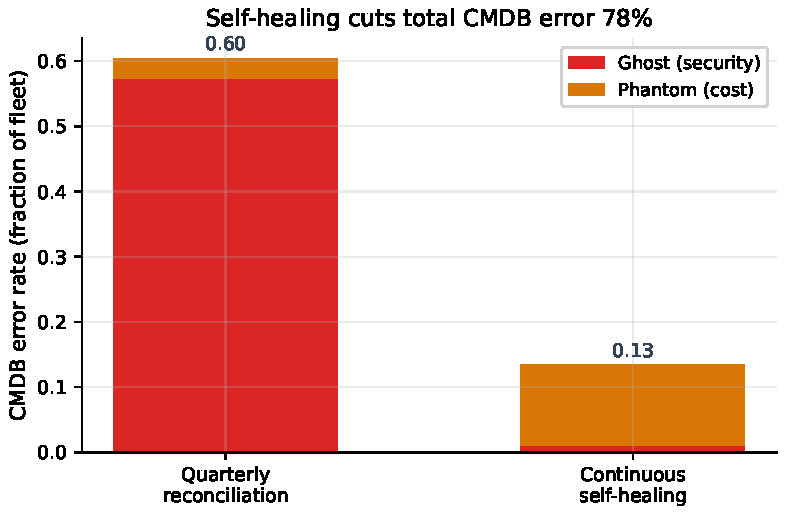
\includegraphics[width=\columnwidth]{fig1_regime.pdf}
\caption{Continuous self-healing reconciliation cuts total CMDB error from 0.6047 under quarterly
reconciliation to 0.1342, a reduction of 0.778, chiefly by removing the discovery-lag ghosts that
dominate the periodic regime.\\[2pt]\textit{Alt text:} A stacked bar chart with two bars; the y-axis is CMDB error rate as a fraction of fleet from 0.0 to 0.6, and each bar splits into a red ghost (security) segment and an orange phantom (cost) segment. The quarterly reconciliation bar totals 0.60 and is almost entirely red ghost error, while the continuous self-healing bar totals 0.13 and is almost entirely orange phantom error.}\label{fig:regime}\end{figure}

\begin{figure}[t]\centering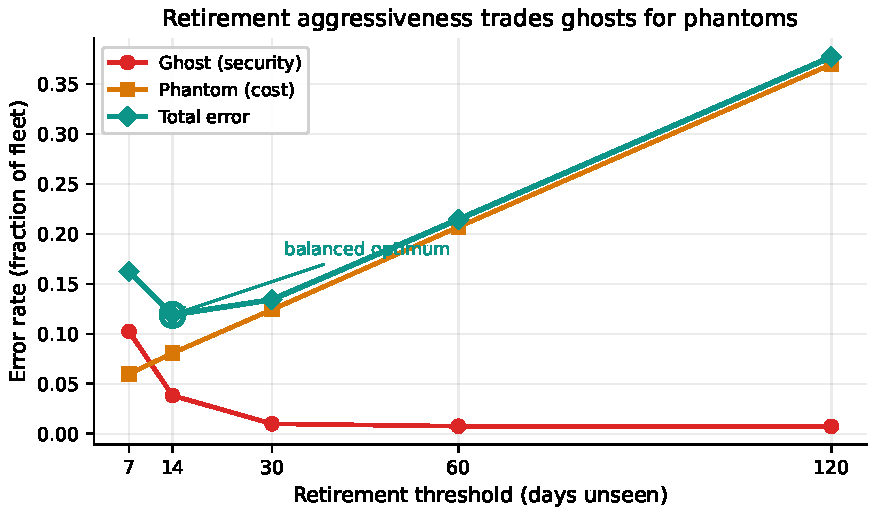
\includegraphics[width=\columnwidth]{fig2_tradeoff.pdf}
\caption{Retirement aggressiveness trades ghost (security) error for phantom (cost) error: as the
threshold lengthens the ghost rate falls and the phantom rate rises, and the total error has an
interior minimum at 14 days.\\[2pt]\textit{Alt text:} A line chart with the retirement threshold in days unseen (7, 14, 30, 60, 120) on the x-axis and error rate as a fraction of fleet on the y-axis. A red ghost (security) curve falls from about 0.10 at 7 days to near 0.01 by 30 days; an orange phantom (cost) curve rises near-linearly from about 0.06 to 0.37; and a teal total-error curve is U-shaped, reaching its marked balanced optimum minimum of about 0.12 at 14 days before climbing to about 0.38 at 120 days.}\label{fig:tradeoff}\end{figure}

\section{Theoretical Analysis}
The four empirical findings are not coincidences of the chosen constants; they follow from the
reconciliation accounting itself. This section derives, in closed form, the ghost-phantom tradeoff,
its interior optimum, the matching-precision floor, and the shift of the cost-weighted optimum, and
checks each derived shape against the frozen numbers of Tables~\ref{tab:threshold}, \ref{tab:precision},
and \ref{tab:cost}. The derivation works at the level of a single representative asset over its
lifetime, because every reported rate is a per-asset Monte Carlo average over the fleet, so the
expected per-asset behavior is exactly what the tables estimate. Throughout, the asset has mean
lifetime $L = 365$ days, a scan runs every cadence $C$ days (here the continuous $C = 1$), a scan
observes the asset with per-scan observability $q$, the retirement threshold is $T$ days, and the
matcher links a fresh observation to the correct record with precision $p$.

\subsection{The ghost rate falls with the threshold}
A ghost is a live asset with no active record. Two mechanisms create one. The first is discovery
lag: a freshly provisioned asset is a ghost until its first observation, which takes a geometric
number of scans with success probability $q$ per scan, so the expected first-observation delay is
about $C / q$ days and contributes a lag component
\begin{equation}
g_{\text{lag}} \;\approx\; \frac{C}{q\,L},
\label{eq:glag}
\end{equation}
the fraction of the lifetime spent undiscovered. This component does not depend on $T$. The second
mechanism is wrongful retirement: a real-but-quiet asset that is missed on every scan for a span
longer than $T$ has its record retired and becomes a ghost until it is observed again. A gap of $T$
days is a run of about $T / C$ consecutive scan misses, each of probability $1 - q$, so the
per-window probability of a wrongful retirement is geometric in the threshold,
\begin{equation}
g_{\text{retire}}(T) \;\approx\; \kappa \,(1 - q)^{T / C},
\label{eq:gretire}
\end{equation}
for a constant $\kappa$ that absorbs the rate at which such windows occur and the time a wrongly
retired asset stays ghosted. The total ghost rate is the sum,
\begin{equation}
g(T) \;\approx\; \frac{C}{q\,L} \;+\; \kappa \,(1 - q)^{T / C},
\label{eq:gtotal}
\end{equation}
and its derivative in $T$ is
\begin{equation}
\frac{dg}{dT} \;\approx\; \frac{\kappa \,\ln(1 - q)}{C}\,(1 - q)^{T / C} \;<\; 0,
\label{eq:dgdt}
\end{equation}
strictly negative because $\ln(1 - q) < 0$. So $g(T)$ decreases with $T$: a longer threshold rarely
deletes a quiet live asset. The decrease is steep at first and then flattens onto the lag floor
$C / (q L)$, which no threshold can remove. This is exactly the shape of the ghost column of
Table~\ref{tab:threshold}: $g$ falls from $0.1025$ at $T = 7$ to $0.0383$ at $14$, $0.0100$ at $30$,
$0.0076$ at $60$, and $0.0075$ at $120$, the last two essentially equal because the wrongful-retirement
term has decayed away and only the lag floor remains. The match is qualitative in $\kappa$ and exact
in shape: monotone decreasing, convex, and asymptoting to a positive floor.

\subsection{The phantom rate rises with the threshold, above a duplicate floor}
A phantom is a record with no live asset behind it, of two kinds. The first kind is a record that
outlives its asset: when an asset is decommissioned, its record is not retired until $T$ further days
of non-observation have passed, so each dead asset leaves a lingering record for about $T$ days,
contributing a linger component proportional to the threshold,
\begin{equation}
\phi_{\text{linger}}(T) \;\approx\; \frac{T}{L},
\label{eq:philinger}
\end{equation}
the lingering record-days per unit of lifetime. The second kind is a duplicate from a failed match.
At each successful observation the matcher fails with probability $1 - p$ and deposits a duplicate
record, which itself persists for about one inter-observation interval $C / q$ before it is
re-matched or retired. Over a lifetime the asset is observed about $q L / C$ times, so the expected
duplicate record-days are about $(1 - p)\,(q L / C)\,(C / q) = (1 - p)\,L$, giving a duplicate
component
\begin{equation}
\phi_{\text{dup}}(p) \;\approx\; (1 - p),
\label{eq:phidup}
\end{equation}
which is independent of $T$: the cadence and the lifetime cancel, leaving the match-failure rate as
the sole driver. The total phantom rate is
\begin{equation}
\phi(T, p) \;\approx\; \frac{T}{L} \;+\; (1 - p),
\label{eq:phitotal}
\end{equation}
with derivative
\begin{equation}
\frac{d\phi}{dT} \;\approx\; \frac{1}{L} \;>\; 0,
\label{eq:dphidt}
\end{equation}
strictly positive: records of gone assets linger about $T$ longer as $T$ grows, while the duplicate
term sits underneath as a $T$-independent offset. The phantom column of Table~\ref{tab:threshold}
rises monotonically, from $0.0598$ at $T = 7$ through $0.0807$, $0.1242$, and $0.2069$ to $0.3696$ at
$T = 120$, the near-linear growth predicted by Eq.~\eqref{eq:philinger} riding on the duplicate offset
of Eq.~\eqref{eq:phidup}.

\subsection{Total error is U-shaped with an interior minimum}
Adding the two, the total error
\begin{equation}
\epsilon(T) \;=\; g(T) + \phi(T) \;\approx\; \frac{C}{q\,L} + \kappa\,(1 - q)^{T/C}
+ \frac{T}{L} + (1 - p)
\label{eq:epstotal}
\end{equation}
is the sum of a strictly decreasing convex term and a strictly increasing linear term, so it is
convex and U-shaped with a unique interior minimizer where the two derivatives cancel,
\begin{equation}
\frac{dg}{dT} + \frac{d\phi}{dT} \;=\; 0
\;\;\Longleftrightarrow\;\;
\frac{\kappa\,\ln(1-q)}{C}\,(1-q)^{T/C} \;+\; \frac{1}{L} \;=\; 0.
\label{eq:foc}
\end{equation}
The left-hand side is negative for small $T$ (the steep ghost decline dominates) and positive for
large $T$ (the ghost term has flattened and the linger term dominates), so a unique interior root
exists. The frozen totals trace exactly this U: $0.1623$ at $T = 7$, falling to $0.1190$ at $14$,
then rising through $0.1342$ at $30$, $0.2145$ at $60$, and $0.3771$ at $120$, with the argmin at
$T = 14$. Neither the most aggressive nor the most lenient threshold is optimal, precisely because
$dg/dT < 0$ and $d\phi/dT > 0$ cannot vanish at an endpoint.

\subsection{Matching precision sets an irreducible floor}
The duplicate term $\phi_{\text{dup}} \approx (1 - p)$ of Eq.~\eqref{eq:phidup} is independent of
both the cadence $C$ and the threshold $T$: it cancelled out of the derivation. It is therefore a
floor on total error that no reconciliation schedule and no retirement policy can cross,
\begin{equation}
\epsilon(T, p) \;\geq\; (1 - p) \quad\text{for all } T, C,
\label{eq:floor}
\end{equation}
and the floor falls linearly as the matcher improves. Holding $T$ at the reference and sweeping $p$,
the total error of Table~\ref{tab:precision} falls from $0.2831$ at $p = 0.80$ to $0.1837$ at $0.90$,
$0.1342$ at $0.95$, and $0.0954$ at $0.99$, tracking the $(1 - p)$ term plus the fixed
threshold-driven residual. The drop from $p = 0.80$ to $p = 0.99$ is $0.1877$, the
duplicate-driven floor proxy reported in the table: it is the portion of the error that is pure
match-failure duplication and that collapses only when the matcher is improved, never when the
cadence or threshold is changed. Equation~\eqref{eq:floor} is the formal statement of the
matching-precision ceiling: $1 - p$ is a hard lower bound that operational tuning cannot reach below.

\subsection{The cost-weighted optimum shifts with the cost ratio}
When ghosts and phantoms are not equally costly, the operating point minimizes the cost-weighted
error of Eq.~\eqref{eq:costweighted}, $\epsilon_w(T) = w_g\,g(T) + w_\phi\,\phi(T)$. Its interior
optimum $T^\star$ solves
\begin{equation}
\frac{d}{dT}\bigl(w_g\,g + w_\phi\,\phi\bigr) \;=\; 0
\;\;\Longleftrightarrow\;\;
w_g \,\frac{dg}{dT} \;=\; -\,w_\phi \,\frac{d\phi}{dT},
\label{eq:costfoc}
\end{equation}
that is, $w_g\,|dg/dT| = w_\phi\,|d\phi/dT|$: the optimum is where the marginal ghost reduction,
priced at $w_g$, exactly offsets the marginal phantom increase, priced at $w_\phi$. Substituting the
two derivatives from Eqs.~\eqref{eq:dgdt} and \eqref{eq:dphidt} gives a closed form for the optimal
threshold,
\begin{equation}
T^\star \;=\; \frac{C}{\ln(1-q)}\,
\ln\!\left(\frac{C}{\kappa\,L\,|\ln(1-q)|}\,\frac{w_\phi}{w_g}\right),
\label{eq:tstar}
\end{equation}
which is increasing in the ratio $w_g / w_\phi$: raising the price of a ghost pushes $T^\star$ up
toward more lenient retirement, and raising the price of a phantom pushes it down toward aggressive
retirement. The frozen optima of Table~\ref{tab:cost} obey exactly this ordering: $T^\star = 30$ days
when ghosts are weighted five to one over phantoms, $14$ days when the two are balanced (recovering
the total-error minimizer of Eq.~\eqref{eq:foc}), and $7$ days when phantoms are weighted five to
one. The optimum moves monotonically and more than fourfold across the weightings, as
Eq.~\eqref{eq:tstar} requires.

\subsection{Summary of the derivation}
Each empirical shape is thus an instance of a structural property: $g(T)$ decreasing onto a discovery-lag
floor (Eq.~\eqref{eq:gtotal}), $\phi(T)$ increasing above a duplicate floor (Eq.~\eqref{eq:phitotal}),
their sum U-shaped with an interior minimum (Eq.~\eqref{eq:foc}) verified at $T = 14$, a hard
matching-precision floor at $1 - p$ (Eq.~\eqref{eq:floor}) verified against the $0.1877$ proxy, and a
cost-weighted optimum (Eq.~\eqref{eq:tstar}) that shifts with $w_g / w_\phi$ and is verified at $30$,
$14$, and $7$ days. The constants $\kappa$, $q$, $C$, and $L$ set the magnitudes, but the four
qualitative findings hold for any positive values of them, which is why we expect them to transfer to
fleets whose absolute rates differ from the model's.

\section{Robustness and Sensitivity}
The model so far treats observability as an exogenous property of an asset. The security-relevant
question is what happens when observability is not exogenous but chosen by an adversary, because the
ghost state is precisely the state an attacker wants its foothold to occupy.

\subsection{The quiet-asset adversary}
Consider an adversary who controls an asset and wants it to escape every inventory-keyed control:
patching, monitoring, scanning, and vulnerability prioritization all read the CMDB, so an asset with
no active record is exempt from all of them. The adversary's lever is observability. By keeping the
asset quiet, powering it down during scan windows, suppressing the discovery agent, or living on a
segment the scanner reaches rarely, the adversary drives its per-scan observability $q$ toward the
low end. From Eq.~\eqref{eq:gretire}, the wrongful-retirement probability $g_{\text{retire}}(T)
\approx \kappa\,(1 - q)^{T/C}$ rises sharply as $q$ falls, because $(1 - q)$ approaches one and the
run of consecutive misses needed to clear the threshold becomes likely rather than rare. The
quiet-asset adversary is therefore manufacturing a ghost on purpose, and once the record is retired
the asset is invisible to every control that trusts the inventory. The model already contains this
worst case: the quiet population in the system model, observed with the low per-scan probability,
is exactly the set of assets an adversary would imitate, and it is the population that the aggressive
$7$-day threshold ghosts at rate $0.1025$ in Table~\ref{tab:threshold}.

\subsection{Setting the threshold for the worst case}
The defensive implication is a direct reading of the cost-weighted optimum. Against the quiet-asset
adversary the cost of a ghost is not a routine inventory inaccuracy but a blind spot that hides a
live threat, so $w_g$ is large relative to $w_\phi$. Equation~\eqref{eq:tstar} then pushes $T^\star$
up: a security-weighted program runs a lenient retirement threshold, accepting more phantom records
in exchange for almost never ghosting a quiet asset. This is the $5 : 1$ row of
Table~\ref{tab:cost}, whose optimum is the lenient $30$-day threshold, against the $7$-day threshold
that a phantom-weighted program would choose. The sensitivity is sharp at the aggressive end: cutting
the threshold from $30$ to $7$ days raises the ghost rate from $0.0100$ to $0.1025$
(Table~\ref{tab:threshold}), a tenfold increase in exactly the error an adversary exploits, while
saving only $0.0644$ of phantom rate. A program that sets its retirement threshold by phantom-cost
considerations alone, chasing a clean inventory, hands the adversary a cheaper path to a ghost. The
worst case must be priced into $w_g$, and the threshold set from the cost-weighted optimum with that
price in mind.

\subsection{Sensitivity of the structural findings}
The extra sweeps needed to see this are already in the frozen tables, so no new table is required.
The retirement-threshold sweep of Table~\ref{tab:threshold} is the ghost sensitivity to threshold
choice; the matching-precision sweep of Table~\ref{tab:precision} is the floor sensitivity to matcher
quality; and the cost-weighted sweep of Table~\ref{tab:cost} is the optimum's sensitivity to the
security-to-cost balance. Across all three, the structural findings are robust to the constants:
the ghost-phantom tradeoff exists whenever retirement can both remove phantoms and delete quiet
assets, the interior optimum follows whenever $dg/dT < 0$ and $d\phi/dT > 0$, the duplicate floor
exists whenever $p < 1$, and the cost-weighted optimum shifts whenever $w_g \neq w_\phi$. An adversary
can move an asset's observability but cannot change the sign of these derivatives, so the operating
guidance, reconcile continuously and set a security-aware retirement threshold, is robust to the
adversarial case as well as the benign one.

\section{Discussion}
Inventory error is two-sided, the two sides are in tension, and the operational guidance follows from
taking that tension seriously rather than chasing a single number to zero.

\emph{Reconcile continuously.} Under periodic reconciliation the dominant error by far is the
discovery-lag ghost: a 90-day cadence leaves a ghost rate of 0.5739, meaning the inventory is blind
to most of the live fleet at any moment, and every control keyed to the inventory inherits that
blindness. Continuous self-healing reconciliation removes almost all of it, cutting total error by
0.778. This is the single largest lever, and it is unambiguous: there is no tradeoff to manage in the
choice of cadence, only error to remove, so the cadence should be as continuous as the discovery
pipeline allows.

\emph{Tune the retirement threshold to an interior optimum.} Once the cadence is continuous, the
residual error is governed by the retirement threshold, and here there is a genuine tradeoff. Too
aggressive a threshold (7 days) deletes real-but-quiet assets and inflates the ghost rate to 0.1025;
too lenient a threshold (120 days) lets records of gone assets linger and inflates the phantom rate
to 0.3696. The total error is minimized at the interior threshold of 14 days, and the practical rule
is to set the retirement threshold deliberately rather than defaulting to whatever the tool ships
with, because both extremes are worse than the interior.

\emph{Invest in the matcher.} Matching precision sets a floor that no cadence and no threshold can
beat. The duplicate phantoms from failed matches form a structural residual, with a floor proxy of
0.1877 at low precision, and the only lever that lowers it is the matcher itself: raising precision
from 0.80 to 0.99 cuts total error by roughly two-thirds. An organization that has already gone
continuous and tuned its threshold but still sees high error should look to its record-linkage
quality, not its schedule. This is where the record-linkage and entity-resolution
literature~\cite{fellegi1969linkage,christen2012matching} pays off operationally.

\emph{Pick the threshold from the mission cost weighting.} Whether 7, 14, or 30 days is right is not
a universal fact but a function of how the organization values a ghost against a phantom. A
security-critical fleet, where an unmanaged asset is the dominant risk, should weight ghosts heavily
and run the lenient 30-day threshold; a cost- or availability-critical fleet, where paying for and
chasing dead records is the dominant pain, should weight phantoms heavily and run the aggressive
7-day threshold; a balanced program lands at 14 days. The retirement threshold is therefore a policy
knob set by the mission, not an engineering constant, and the cost-weighted objective in
Eq.~\eqref{eq:costweighted} is the right lens for setting it.

\section{Threats to Validity}
\emph{Construct validity.} The model abstracts fleet churn as exponential lifetimes with steady-state
arrivals and probabilistic observation, and matching as a single per-observation precision. Real
churn may be bursty, correlated with asset type, or seasonal around procurement and refresh cycles,
and real matching precision varies with the attributes available to the linker. These would shift the
absolute ghost and phantom rates but not the structural relationships: a ghost-phantom tradeoff exists
whenever retirement can both remove phantoms and delete quiet assets, an interior optimum follows from
the two errors moving oppositely, and a duplicate-driven floor exists whenever matching precision is
below one.

\emph{Internal validity.} Because the study is pre-registered and the evaluation seeds were inspected
only once, the reported numbers are not the product of analytic search. The development of the model
used separate seeds, and no parameter was tuned to clear a threshold. The mechanical evaluation
script computes each verdict from the frozen data with no hand-set value.

\emph{External validity.} The mean lifetime, the observability, the cadences, and the threshold and
precision sweeps are documented priors, not measurements from any organization, so the absolute
magnitudes (a quarterly ghost rate of 0.5739, a continuous total error of 0.1342) should be read as
illustrative of the model rather than as field estimates. The comparative findings, the regime
reduction, the interior optimum, the matching-precision floor, and the cost-weighted shift, depend on
the qualitative structure of the model rather than on the specific constants, and we expect them to
transfer. Calibrating the fleet dynamics, observability, and matching precision against a real
inventory and reconciliation record is the natural next step and would convert the illustrative
magnitudes into estimates.

\emph{Statistical validity.} Intervals are BCa bootstrap intervals over 25 seeds, appropriate for the
small-sample, possibly skewed statistics reported here; we use interval non-overlap rather than
significance testing throughout, avoiding the multiple-comparison pitfalls of repeated $p$-values.
The ghost and phantom costs are different in kind and are reported separately, with the cost-weighted
view offered as a parameterized lens rather than a single universal score.

\section{Conclusion}
A configuration management database is the inventory on which security and cost management both rest,
and its errors are two-sided: ghosts, the live assets the inventory cannot see, are a security cost,
and phantoms, the records with no real asset behind them, are a financial and noise cost. In a
pre-registered simulation of a churning fleet, continuous self-healing reconciliation cut total
inventory error from 0.6047 under quarterly reconciliation to 0.1342, a reduction of 0.778, almost
all of it by closing the discovery lag that turns new assets into ghosts. The two errors trade off
against retirement aggressiveness, so total error has an interior minimum at a 14-day threshold rather
than at either extreme; matching precision sets a floor, with total error falling from 0.2831 to
0.0954 as precision rises from 0.80 to 0.99 against a duplicate-driven floor proxy of 0.1877; and the
cost-minimizing threshold shifts from 30 days when ghosts are weighted five to one, to 14 days when
balanced, to 7 days when phantoms are weighted five to one. The deployment guidance is concrete:
reconcile continuously, tune the retirement threshold to the interior optimum set by the
security-to-cost balance, and invest in the matcher, because matching precision sets a floor that no
cadence can beat. Calibrating the model against a real inventory and reconciliation record is the
next step toward turning these structural findings into field estimates.

\section*{Data Availability Statement}
The data and code that support the findings of this study are openly available in the research-papers repository at \url{https://github.com/Harshavardhanmalla-Labs/research-papers/tree/main/paper19}. The manuscript sources, figures, analysis code, and frozen result tables are included and regenerate every reported number deterministically from the fixed seeds.

\section*{Disclosure Statement}
No potential conflict of interest was reported by the author.

\section*{Funding}
No funding was received.

% Generated by IEEEtran.bst, version: 1.14 (2015/08/26)
\begin{thebibliography}{10}
\providecommand{\url}[1]{#1}
\csname url@samestyle\endcsname
\providecommand{\newblock}{\relax}
\providecommand{\bibinfo}[2]{#2}
\providecommand{\BIBentrySTDinterwordspacing}{\spaceskip=0pt\relax}
\providecommand{\BIBentryALTinterwordstretchfactor}{4}
\providecommand{\BIBentryALTinterwordspacing}{\spaceskip=\fontdimen2\font plus
\BIBentryALTinterwordstretchfactor\fontdimen3\font minus
  \fontdimen4\font\relax}
\providecommand{\BIBforeignlanguage}[2]{{%
\expandafter\ifx\csname l@#1\endcsname\relax
\typeout{** WARNING: IEEEtran.bst: No hyphenation pattern has been}%
\typeout{** loaded for the language `#1'. Using the pattern for}%
\typeout{** the default language instead.}%
\else
\language=\csname l@#1\endcsname
\fi
#2}}
\providecommand{\BIBdecl}{\relax}
\BIBdecl

\bibitem{nist80053}
{Joint Task Force}, ``Security and privacy controls for information systems and
  organizations,'' National Institute of Standards and Technology, Tech. Rep.
  NIST Special Publication 800-53 Rev. 5, 2020.

\bibitem{cisabod2301}
{Cybersecurity and Infrastructure Security Agency (CISA)}, ``Binding
  operational directive 23-01: Improving asset visibility and vulnerability
  detection on federal networks,'' U.S. Department of Homeland Security, Tech.
  Rep., Oct. 2022,
  \url{https://www.cisa.gov/news-events/directives/bod-23-01-improving-asset-visibility-and-vulnerability-detection-federal-networks}.

\bibitem{nist80137}
K.~Dempsey, N.~S. Chawla, A.~Johnson, R.~Johnston, A.~C. Jones, A.~Orebaugh,
  M.~Scholl, and K.~Stine, ``Information security continuous monitoring (iscm)
  for federal information systems and organizations,'' National Institute of
  Standards and Technology, Tech. Rep. NIST Special Publication 800-137, 2011.

\bibitem{nist80137a}
K.~Dempsey, V.~Pillitteri, C.~Baer, R.~Niemeyer, R.~Rudman, and S.~Urban,
  ``Assessing information security continuous monitoring (iscm) programs:
  Developing an iscm program assessment,'' National Institute of Standards and
  Technology, Tech. Rep. NIST Special Publication 800-137A, 2020.

\bibitem{fellegi1969linkage}
I.~P. Fellegi and A.~B. Sunter, ``A theory for record linkage,'' \emph{Journal
  of the American Statistical Association}, vol.~64, no. 328, pp. 1183-1210,
  1969.

\bibitem{christen2012matching}
P.~Christen, \emph{Data Matching: Concepts and Techniques for Record Linkage,
  Entity Resolution, and Duplicate Detection}.\hskip 1em plus 0.5em minus
  0.4em\relax Springer, 2012.

\bibitem{kephart2003vision}
J.~O. Kephart and D.~M. Chess, ``The vision of autonomic computing,''
  \emph{IEEE Computer}, vol.~36, no.~1, pp. 41-50, 2003.

\bibitem{efron1987bca}
B.~Efron, ``Better bootstrap confidence intervals,'' \emph{Journal of the
  American Statistical Association}, vol.~82, no. 397, pp. 171-185, 1987.

\bibitem{efron1994introduction}
B.~Efron and R.~J. Tibshirani, \emph{An Introduction to the Bootstrap}.\hskip
  1em plus 0.5em minus 0.4em\relax Chapman \& Hall/CRC, 1994.

\bibitem{wohlin2012experimentation}
C.~Wohlin, P.~Runeson, M.~H{\"o}st, M.~C. Ohlsson, B.~Regnell, and
  A.~Wessl{\'e}n, \emph{Experimentation in Software Engineering}.\hskip 1em
  plus 0.5em minus 0.4em\relax Springer, 2012.

\bibitem{paper10autoheal}
H.~Malla, ``{AutoHeal}: A self-healing framework for cyber-hygiene remediation
  on government endpoint fleets,''
  \url{https://github.com/Harshavardhanmalla-Labs/research-papers/tree/main/paper10},
  2026, companion paper; source, code, and frozen results in the same
  repository.

\bibitem{fips199}
{National Institute of Standards and Technology}, ``Standards for security
  categorization of federal information and information systems,'' U.S.
  Department of Commerce, Tech. Rep. FIPS PUB 199, 2004.

\bibitem{bertino2005database}
E.~Bertino and R.~Sandhu, ``Database security-concepts, approaches, and
  challenges,'' \emph{{IEEE} Transactions on Dependable and Secure Computing},
  vol.~2, no.~1, pp. 2-19, 2005.

\bibitem{verizon2026dbir}
{Verizon}, ``2026 data breach investigations report ({DBIR}),'' Verizon
  Business, Tech. Rep., 2026,
  \url{https://www.verizon.com/business/resources/reports/dbir/}.

\bibitem{paper4hygieneprio}
H.~Malla, ``{HygienePrio}: Cyber-hygiene signal augmentation for
  {EPSS}-weighted vulnerability prioritization,''
  \url{https://github.com/Harshavardhanmalla-Labs/research-papers/tree/main/paper4},
  2026, companion paper; source, code, and frozen results in the same
  repository.

\end{thebibliography}

\end{document}
